\documentclass{scrartcl}

\usepackage{tikz}
\usetikzlibrary{matrix.skeleton}
\usetikzlibrary{positioning}

\usepackage[justification=centering,labelfont={sf,bf,up},labelsep=period,font=small]{caption}
\captionsetup[figure]{position=bottom,singlelinecheck=false}
\usepackage{float}
\floatstyle{komabelow}
\restylefloat{figure}


\usepackage{hyperref}

\tikzset{highlight/.style={draw=#1!75, fill=#1!25, rounded corners=1pt}}

\title{\texttt{matrix.skeleton}'s Regression Tests}
\author{}
\date{}

\begin{document}

\maketitle

This document serves as a basic regression test suite for \texttt{matrix.skeleton}.
It was introduced to validate the multiple-matrix support implementation.
As a starting point, the only expectation is that the examples have highlights that \textit{look right}.


\begin{figure}[h]
\centering
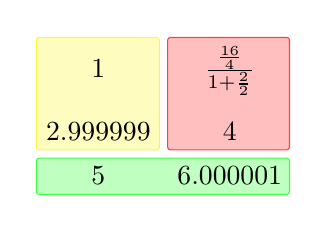
\begin{tikzpicture}
\matrix (m) [matrix of math nodes, column sep = 3pt, row sep = 3pt, label skeleton] {
1        & \frac{\frac{16}{4}}{1 + \frac{2}{2}} \\
2.999999 & 4                                    \\
5        & 6.000001                             \\
};

\fitandstyle[background]{(m-cell-1-1) (m-cell-2-1)}{highlight = yellow}
\fitandstyle[background]{(m-cell-1-2) (m-cell-2-2)}{highlight = red}
\fitandstyle[background]{(m-cell-3-1) (m-cell-3-2)}{highlight = green}
\end{tikzpicture}
\caption{Single matrix}
\end{figure}


\begin{figure}[h]
\centering
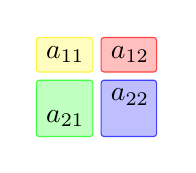
\begin{tikzpicture}
\matrix (m) [matrix of math nodes, column sep = 3pt, row sep = 3pt, label skeleton] {
a_{11} & a_{12} \\
|[anchor=north]| a_{21} & a_{22} \\
};

\fitandstyle[background]{(m-cell-1-1)}{highlight = yellow}
\fitandstyle[background]{(m-cell-1-2)}{highlight = red}
\fitandstyle[background]{(m-cell-2-1)}{highlight = green}
\fitandstyle[background]{(m-cell-2-2)}{highlight = blue}
\end{tikzpicture}
\caption{Single matrix using a non-base anchor}
\end{figure}


\begin{figure}[h]
\centering
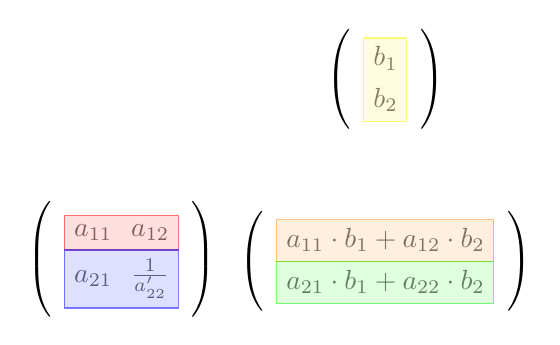
\begin{tikzpicture}

\tikzset{my-matrix/.style={matrix of math nodes, label skeleton,
                           left delimiter=(, right delimiter =)}}

\matrix (A) [my-matrix] {
  a_{11} & a_{12} \\
  a_{21} & \frac{1}{a'_{22}} \\
};
\matrix (C) [my-matrix, right= of A] {
  a_{11} \cdot b_1 + a_{12} \cdot b_2 \\
  a_{21} \cdot b_1 + a_{22} \cdot b_2 \\
};
\matrix (B) [my-matrix, above=of C] {
  b_1 \\
  b_2 \\
};

\fitandstyle{(A-row-1)}{draw=red, fill=red!25, opacity=0.5}
\fitandstyle{(A-row-2)}{draw=blue, fill=blue!25, opacity=0.5}
\fitandstyle{(B-column-1)}{draw=yellow, fill=yellow!25, opacity=0.5}
\fitandstyle{(C-cell-1-1)}{draw=orange, fill=orange!25, opacity=0.5}
\fitandstyle{(C-cell-2-1)}{draw=green, fill=green!25, opacity=0.5}

\end{tikzpicture}
\caption{Multiple matrices}
\end{figure}


\end{document}
